% IMPOSTAZIONI DOCUMENTO 

\documentclass[a4paper, english]{article}

\usepackage[citestyle=numeric,bibstyle=numeric,maxcitenames=1,useprefix,hyperref,natbib,backend=bibtex]{biblatex}
\usepackage[utf8]{inputenc}
\usepackage{babel}
\usepackage{uniudtesi}
\usepackage[nottoc]{tocbibind}
\usepackage{indentfirst}
\usepackage[counterclockwise]{rotating}
\usepackage{listings}
\usepackage{fancyhdr}
\usepackage{longtable}
\usepackage{subcaption}
\usepackage{multirow}
\usepackage{csquotes}
\usepackage{booktabs}
\usepackage{quoting}
\usepackage{listings}
\usepackage{amsmath}
\usepackage{adjustbox}
\usepackage{array}
\usepackage{amsmath,amsfonts,amssymb,amsthm}
\usepackage{latexsym}
\usepackage{caption}
\usepackage{changepage}
\usepackage{enumitem}
\usepackage{threeparttable}
\usepackage{fancyvrb}
\usepackage{makecell}
\usepackage{tocloft}
\usepackage{xstring}
\usepackage{mathtools}
\usepackage{etoolbox}
\usepackage{xcolor,colortbl}
\usepackage{lscape}
\usepackage{algorithm}
\usepackage{algpseudocode}
\usepackage{hyperref}
\usepackage{titlesec}

% NOME DEL FILE CONTENENTE LA BIBLIOGRAFIA. IL FILE DEVE TROVARSI NELLA ROOT DEL FILE .TEX, AVERE IL NOME INDICATO TRA LE PARENTESI GRAFFE ED ESTENSIONE .bib 

\bibliography{bibliography}

% PATH RELATIVO DALLA ROOT DEL FILE TEX ALLA CARTELLA CONTENENTE LE IMMAGINI

\graphicspath{{./immagini/}}

\raggedbottom

% IMPOSTAZIONI FONT 

\renewcommand{\baselinestretch}{1.2}

% OPZIONE CHE CONSENTE DI SPEZZARE LE URL IN QUALUNQUE LORO PUNTO

\expandafter\def\expandafter\UrlBreaks\expandafter{\UrlBreaks
\do\a\do\b\do\c\do\d\do\e\do\f\do\g\do\h\do\i\do\j
\do\k\do\l\do\m\do\n\do\o\do\p\do\q\do\r\do\s\do\t
\do\u\do\v\do\w\do\x\do\y\do\z\do\A\do\B\do\C\do\D
\do\E\do\F\do\G\do\H\do\I\do\J\do\K\do\L\do\M\do\N
\do\O\do\P\do\Q\do\R\do\S\do\T\do\U\do\V\do\W\do\X
\do\Y\do\Z}

% COLONNE TABELLA DIMENSIONE FISSATA 

\newcolumntype{L}[1]{>{\raggedright\let\newline\\\arraybackslash\hspace{0pt}}m{#1}}
\newcolumntype{C}[1]{>{\centering\let\newline\\\arraybackslash\hspace{0pt}}m{#1}}
\newcolumntype{R}[1]{>{\raggedleft\let\newline\\\arraybackslash\hspace{0pt}}m{#1}}

% NO VIRGOLETTE IN BIBLIOGRAFIA

\DeclareFieldFormat[inbook]{title}{#1} 
\DeclareFieldFormat[inproceedings]{title}{#1} 
\DeclareFieldFormat[article]{title}{#1}

% DEFINIZIONE DI MACRO

\newcommand{\N}{\mathbb{N}}

% LSTLISTINGS CON LINE WRAPPING

\lstset{
basicstyle=\small\ttfamily,
columns=flexible,
breaklines=true
}

% VISUALIZZAZIONE DI FILE JSON

\colorlet{punct}{red!60!black}
\definecolor{background}{HTML}{EEEEEE}
\definecolor{delim}{RGB}{20,105,176}
\colorlet{numb}{magenta!60!black}


\lstdefinelanguage{json}{
    basicstyle=\normalfont\ttfamily,
    numbers=left,
    numberstyle=\scriptsize,
    stepnumber=1,
    numbersep=8pt,
    showstringspaces=false,
    breaklines=true,
    frame=lines,
    backgroundcolor=\color{background},
    literate=
     *{0}{{{\color{numb}0}}}{1}
      {1}{{{\color{numb}1}}}{1}
      {2}{{{\color{numb}2}}}{1}
      {3}{{{\color{numb}3}}}{1}
      {4}{{{\color{numb}4}}}{1}
      {5}{{{\color{numb}5}}}{1}
      {6}{{{\color{numb}6}}}{1}
      {7}{{{\color{numb}7}}}{1}
      {8}{{{\color{numb}8}}}{1}
      {9}{{{\color{numb}9}}}{1}
      {:}{{{\color{punct}{:}}}}{1}
      {,}{{{\color{punct}{,}}}}{1}
      {\{}{{{\color{delim}{\{}}}}{1}
      {\}}{{{\color{delim}{\}}}}}{1}
      {[}{{{\color{delim}{[}}}}{1}
      {]}{{{\color{delim}{]}}}}{1},
}

\makeatletter
\renewcommand{\ALG@name}{Listing}
\renewcommand{\listalgorithmname}{List of Listings}
\makeatother

\titleclass{\subsubsubsection}{straight}[\subsection]

\newcounter{subsubsubsection}[subsubsection]
\renewcommand\thesubsubsubsection{\thesubsubsection.\arabic{subsubsubsection}}
\renewcommand\theparagraph{\thesubsubsubsection.\arabic{paragraph}} % optional; useful if paragraphs are to be numbered

\titleformat{\subsubsubsection}
  {\normalfont\normalsize\bfseries}{\thesubsubsubsection}{1em}{}
\titlespacing*{\subsubsubsection}
{0pt}{3.25ex plus 1ex minus .2ex}{1.5ex plus .2ex}

\makeatletter
\renewcommand\paragraph{\@startsection{paragraph}{5}{\z@}%
  {3.25ex \@plus1ex \@minus.2ex}%
  {-1em}%
  {\normalfont\normalsize\bfseries}}
\renewcommand\subparagraph{\@startsection{subparagraph}{6}{\parindent}%
  {3.25ex \@plus1ex \@minus .2ex}%
  {-1em}%
  {\normalfont\normalsize\bfseries}}
\def\toclevel@subsubsubsection{4}
\def\toclevel@paragraph{5}
\def\toclevel@paragraph{6}
\def\l@subsubsubsection{\@dottedtocline{4}{7em}{4em}}
\def\l@paragraph{\@dottedtocline{5}{10em}{5em}}
\def\l@subparagraph{\@dottedtocline{6}{14em}{6em}}
\makeatother

\setcounter{secnumdepth}{4}
\setcounter{tocdepth}{4}

% INFORMAZIONI GENERALI

\titolo{Readersourcing 2.0\\Technical Documentation}
\nomeprogetto{MICHAEL SOPRANO AND STEFANO MIZZARO}

\begin{document}

\maketitle

\tableofcontents

\newpage

\listoffigures

\newpage

\listoftables

\newpage

\section{Introduction}

This technical documentation provides an overview of the \emph{Readersourcing 2.0} ecosystem. Initially, a recap of its general architeture is presented and subsequently, for each of its components, a brief recap of their role and purpose is presented along with some specific aspects, such as the technology used, the internal architecture, the structure of the database and more. This is done by using different types of diagrams belonging to the UML standard (unless otherwise specified) which are drew according to the set of style rules for that standard proposed by \citet{Fowler03}.

\section{General Architecture}

Readersourcing 2.0 is an ecosystem composed of more than one application. Indeed, there must be one application that acts as a server to gather all the ratings given by readers and one that acts as a client to allow readers to effectively rate publications. There is one additional component since the task of editing files encoded in PDF format is carried out by an ad hoc software library exploited by the server side application. An overview of the architecture of Readersourcing 2.0 is shown in Figure~\ref{fig:architecture} and in the following we briefly describe these three components. 

\begin{figure}[h]
\centering
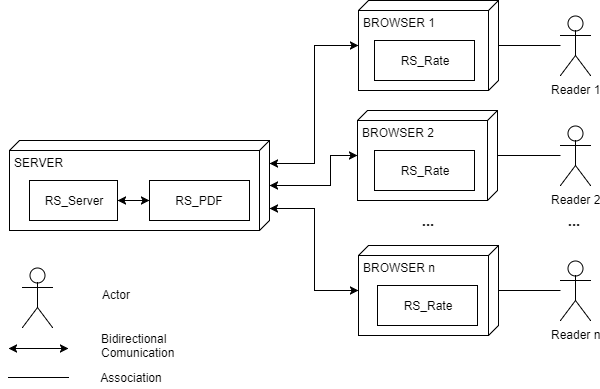
\includegraphics[width=\textwidth]{figures/architecture.png}
\caption{Architecture of Readersourcing 2.0 (NOT UML).}
\label{fig:architecture}
\end{figure}

\section{RS\_Server}

\emph{RS\_Server} is the server-side application which has the task to collect and aggregate the ratings given by readers and to use RSM and TRM to compute quality scores for readers and publications. RS\_Server must be deployed on a machine along with an instance of RS\_PDF, otherwise it can not work properly.
Then, there are up to \emph{n} different browsers, with the corresponding end-users, which communicate with the server: each of them has an instance of \emph{RS\_Rate}, which is the true client. 
Both RS\_PDF and RS\_Rate are described in the following. 
This setup means that every interaction between readers and server is carried out through clients installed on readers' browsers and these clients have to handle the registration and authentication of readers, the rating action and the download action of link-annotated publications.

During the design phase of RS\_Server some strategies have been adopted to ensure its extensibility and generality. This means that: (i) it is straightforward to add new models, (ii) each model shares the same input data format, and (iii) if a model needs to save values locally to the RS\_Server (i.e., in its database), there is a standard procedure to allow that.

\subsection{Implementation and Technology}

RS\_Server is developed in Ruby on Rails,\footnote{\url{https://rubyonrails.org/}} which is a framework that
The technology used to develop RS\_Server is an open-source web application framework called \emph{Ruby on Rails} (it is also called \emph{RoR} or \emph{Rails} only; more specifically, \emph{Rails} is the framework built above \emph{Ruby}, the actual programming language). It allows to build applications strongly based on the Model-View-Controller (MVC) architectural pattern.

The MVC pattern allows to separate the control logic of the program from data  presentation and business logic. Thefore, it allows to obtain an effective architecture since the first moments of its design phase. An intuitive representation of the structure that this pattern allows to obtain is shown in Figure \ref{fig:mvc}. This structure consists of three distinct entities, called \emph{Controller}, \emph{Model} and \emph{View}. These entities have the task of, respectively, managing control logic, encapsulating business logic and implementing data presentation.

\begin{figure}[!tbp]
\centering
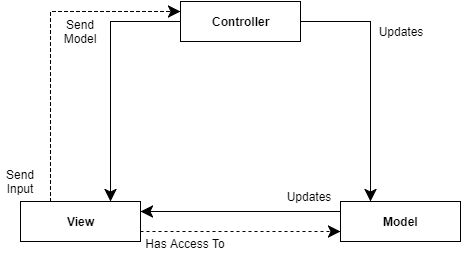
\includegraphics[scale=0.7]{figures/mvc.png}
\caption{Intuitive scheme of the MVC pattern (NOT UML).}
\label{fig:mvc}
\end{figure}

The Controller has direct access to the Model and to the View; from the latter, generally, it receives the user input and on its basis the Controller itself updates the internal state of the Model using its methods. Finally, the Controller sends the updated Model to the View, which is then exploited by the View itself to obtain and display the results of the processing. A generic software can have more than one Controller, where each of them can manage more than one Model instances. In MVC frameworks dedicated to the development of web applications such as Rails, in fact, it is common practice to have a number of Controllers equal to the number of entities modeled within the application domain. Furthermore, there may be more than one View implementation to present the internal state of a specific type of Model.

The use of MVC pattern is not the only founding principle of Rails. One of the most important principles on which Rails itself is based for the developement of quality applications is \lq\lq Convention Over Configuration\rq\rq{}. In other words, the framework tries to minimize the decisions that the developer must take during the construction of its application by adopting standard conventions that he can modify if he needs more flexibility. The founding principles of Rails can be deepened by reading the \emph{Rails Doctrine}\footnote{\url{https://rubyonrails.org/doctrine/}}.

As a last note, Rails is a continuously developing framework and is used industrially by several well-known industry players such as \emph{GitHub}, \emph{SoundCloud}, \emph{Airbnb} and others. It is, therefore, a widespread and appreciated technology, for which there is an active community and a lot of learning material.

\subsection{Communication Paradigm}

A modern MVC framework such as Rails allows to develop various kind of web applications. One of the possibilities is to create a \emph{Web Service}, which is a software component capable of carrying out various operations made remotely available through the exchange of messages encoded in a standard interchange format such as \emph{JSON}, all thanks to a transport layer built above the basic Internet protocols like \emph{HTTP}. All this, however, must be carried out according to a paradigm that defines precisely what are the functionalities (resources and operations) actually available and which messages must be received in order to access them.

One of the possible communication paradigms for Web Services is \emph{RESTful} (\emph{REpresentational State Transfer}). Within this paradigm, the functionalities of a Web Service are represented by resources identified by different URIs and the type of HTTP message sent establishes the operation to be performed. The result of the operation initiated by the message received from the Web Service is a new message encoded according to same interchange format of the one which has been sent and it is the client's responsibility to correctly interpret and use the response of the Web Service itself.

RS\_Server is a Web Service (Server API-Only, according to Rails terminology) based on a communication paradigm composed of RESTful (REpresentational State Transfer) interfaces and on the exchange of messages encoded in JSON format through the transport layer provided by the HTTP protocol.

The communication interface of RS\_Server is constantly evolving and, for this reason, it makes no sense to fully include it in this document. However, it is possible to consult it freely and to see examples of requests that can be made by visiting the URL below.

\begin{table}[h]
\centering
\begin{tabular}{p{12cm}}
  \toprule
	\url{https://web.postman.co/collections/4632696-c26fc049-7021-4691-beb3-97cebfb60adb?workspace=8a3ef37e-60b1-4b49-8782-e73d2a6e3a8c}  \\
 \toprule
  \end{tabular}
\end{table}

To provide an example, a subset of the RESTFul interface of RS\_Server is shown in Table \ref{tab:rest}. These operations are all those available to handle one of the entities of the application domain, namely the publications. Let's then suppose that a user triggers a show operation for a publications characterized by an identifier equal to 1 by visiting the corresponding endpoint. The JSON-encoded response of RS\_Server would be something like the one below.

\begin{lstlisting}[language=json,firstnumber=1]
{
  "id": 1,
  "doi": "10.1140/epjc/s10052-018-6047-y",
  "title": "Uncertainties in WIMP dark matter scattering revisited",
  "author": "John Ellis",
  "creator": "Springer",
  "producer": null,
  "...": ...,
  "created_at": "2018-08-02T13:27:46.988Z",
  "updated_at": "2018-08-02T13:27:49.135Z",
  "...": ...,
}
\end{lstlisting}

\begin{table}
\centering
\begin{threeparttable}
\begin{tabular}{p{4cm}C{1.5cm}C{1.8cm}p{6cm}}
\toprule
\textbf{Endpoint}  &\textbf{HTTP Message} & \textbf{Operation} & \textbf{Description} \\
\midrule
/publications.json & GET & Index & Fetches the entire collection of Publications. \\
/publications/1.json & GET & Show & Returns the Publication with identifier equal to 1. \\
/publications/lookup.json & POST & Lookup & Searches for a Publication; if it doesn't exists, it is fetched from the given URL. \\
/publications/random.json & GET & Random & Returns a random Publication. \\ 
/publications/1/is\_rated.json & GET & Is Rated & Checks if the Publication with identifier equal to 1 has been rated by at least one reader. \\
/publications.json & POST & Create & Creates a new Publication. \\
/publications/fetch.json & POST & Fetch & Fetches a Publication from the given URL. \\
/publications/refresh.json & GET & Refresh & Fetches again an existing Publication. \\
/publications/1.json & PUT & Update & Updates the Publication with identifier equal to 1. \\
/publications/1.json & DELETE & Delete & Deletes the Publication with identifier equal to 1.\\
\dots & \dots & \dots & \dots \\
\bottomrule
\end{tabular}
\caption{Subset of the RESTFul interface of RS\_Server.}
\label{tab:rest}
 \end{threeparttable}
\end{table}

\subsection{Database}

To implement the storage of edited publications, user authentication and the other functionalities it is necessary to define the structure of a database, which is indeed shown in Figure \ref{fig:er}. There are three entities modeled within the application domain of Readersourcing 2.0:

\begin{itemize}
\item \textbf{Users}: models the users of the system itself, which are characterized by their personal data, an optional \emph{ORCID} a boolean used to check if the user wants to receive mail or not. There are also some attributes used to store various kind of tokens to allow operations like password reset;
\item \textbf{Ratings}: models the ratings given by readers of publications which are characterized by a score;
\item \textbf{Publications}: models the publications rated by their readers which are characterized by an optional \emph{DOI}, by various metadata and by a whole series of attributes used to manage the paths on the server filesystem in order to guarantee a correct storage of the original and edited files encoded in PDF format. 
\end{itemize}
Moreover, each of these entities is characterized by further attributes (\emph{steadiness}, \emph{informativeness}, \dots) which represent the scores/parameters computed by the Readersourcing models.

\begin{figure}[!tbp]
\centering
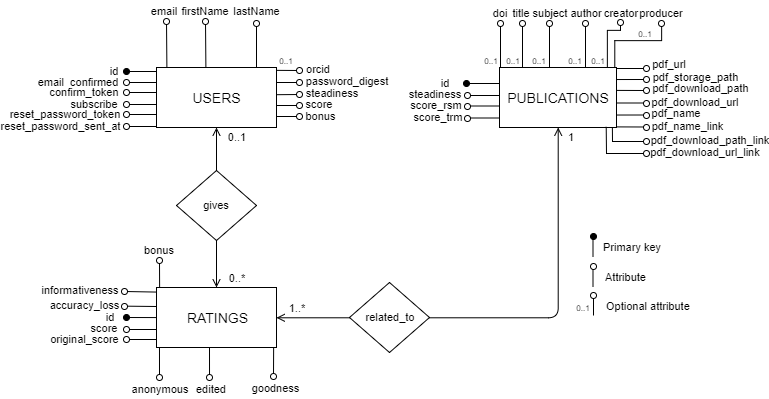
\includegraphics[width=\textwidth]{figures/er.png}
\caption{Entity-Relationship schema of the database of RS\_Server (NOT UML).}
\label{fig:er}
\end{figure}

In the schema shown in Figure \ref{fig:er} are also represented two relationships (\emph{gives} and \emph{related\_to}) that exist between these three entities. These relationships allow to \lq\lq tie together\rq\rq{} the entities to which they refer and they ensure compliance with the \emph{referential integrity} constraint.

In particular, the \emph{gives} relation establishes that a user can give $[0,\dots ,n]$ different ratings, while a single rating can be expressed at most by a user. At first glance, the multiplicity equal to $0$ described by the schema shown in Figure \ref{fig:er} regarding users may seem strange. The meaning of this constraint is to allow the expression of anonymous ratings. Likewise, the relation \emph{related\_to} establishes that a rating is relative to a certain  publication, while a publication can be characterized by $[1,\dots ,n]$ different ratings. Moreover, this structure allows to comply in a \lq\lq natural\rq\rq{} way with other constraints, such as the fact that if at least at least one publication does not exist, no ratings have to exist.

\subsection{Class Diagram}

Figure \ref{fig:class-1} shows a diagram of the main classes of RS\_Server. As one can see, the convention for which there is an MVC triple for each of the entities modeled in the application domain is followed, althought Views are not shown in the diagram because in this case they are just methods. The Controller methods represent actions that a user can perform on individual entities or on collections of them, thus mapping the endpoints of the communication protocol used in order to allow the communication between RS\_Server and the instances of RS\_Rate. As for the Models, their attributes represent the characteristics of the reference entity, while their methods encapsulate the business logic.

Furthermore, there are two additional Controllers\footnote{\emph{Application Controller} and \emph{AuthenticationController}} responsible for managing user authentication. RS\_Server, as specified previously, is a Web Service; this means that the user interface is presented directly on the instances of RS\_Rate and, therefore, those instances send messages to which RS\_Server responds once the necessary processing has been completed, according to the RESTful communication paradigm. Because of this design choice, it is not possible to use the \lq\lq classic\rq\rq{} server-side approach to user authentication according to which some information relative to the logged user are saved in the session data, since RESTful paradigm is \emph{stateless}. To be able to authenticate himself, therefore, the user client must attach to each request a \emph{token} that identifies its user as valid within the system. Therefore, a \emph{token-based} authentication approach has been implemented.

When a user performs the first request to RS\_Server since some time, he must fill in the login form. If these inserted credentials exist in the database they are encrypted (a \emph{payload} is obtained) and used together with a unique \emph{signature} to create an alphanumeric JSON string, i.e. the actual token, a copy of which is saved inside the database. This token thus generated is sent to the RS\_Rate instance of the user itself which stores it in a secure cookie characterized by an expiration date after which the procedure must be repeated. At each subsequent request to RS\_Sever, the instance of RS\_Rate attaches\footnote{In the \emph{Authorization} header of the HTTP package} the previously obtained token in order to demonstrate that its user has successfully completed the authentication procedure. As for RS\_Server, if a token is present it is extracted and decoded and if it corresponds to one of those saved in the database, then the user identified by the payload is authorized to proceed. An intuitive scheme of the process procedure is shown in Figure \ref{fig:auth}.

\begin{figure}[!tbp]
\centering
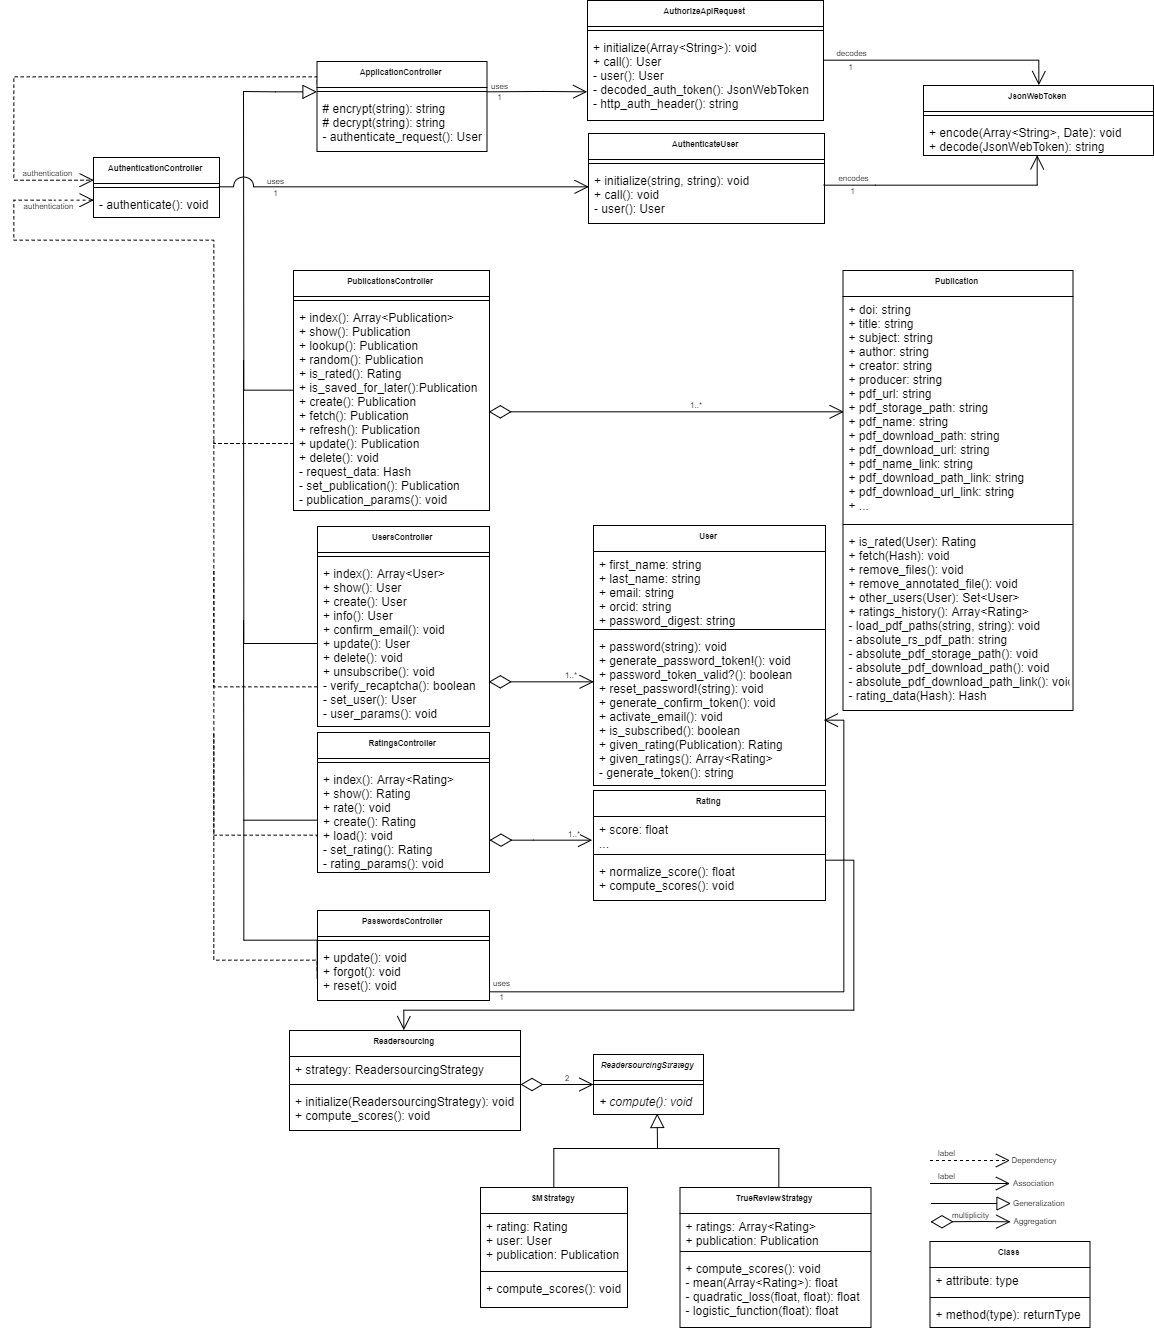
\includegraphics[scale=0.4]{figures/classi-1.png}
\caption{Class diagram of RS\_Server.}
\label{fig:class-1}
\end{figure}

\begin{figure}[!tbp]
\centering
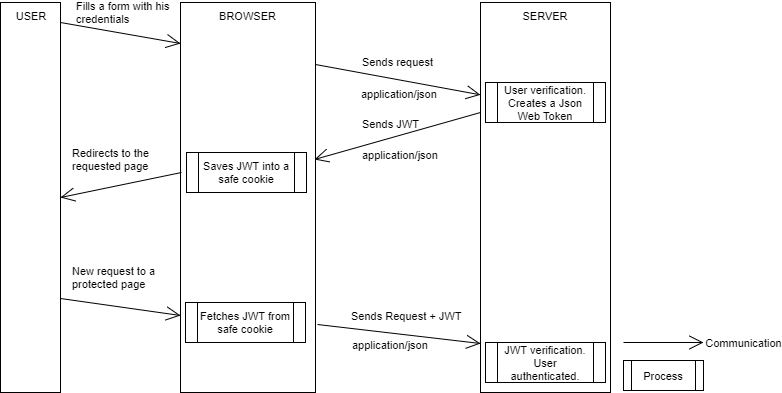
\includegraphics[width=\textwidth]{figures/autenticazione.png}
\caption{Representation of the token-based authentication process (NOT UML).}
\label{fig:auth}
\end{figure}

Finally, there is an additional set of classes which are used for different purposes than representing MVC triples for the entitities of the application domain. In particular, they are exploited internally by the model containing the business logic to manage the given ratings and have the task of implementing the Readersourcing models. The structure of these classes follows a design pattern called\footnote{\emph{Readersourcing}, \emph{ReadersourcingStrategy}, \emph{SMStrategy} e \emph{TrueReviewStrategy}. } \emph{Strategy} because this pattern allows to integrate new models at a later time without having to make radical changes in the structure of RS\_Server.

\subsection{Deploy}

There are three main modalities that can be exploited to deploy a working instance of RS\_Server in \emph{development} or \emph{production} environment. The former environment must be used if there is the need to add custom Readersourcing model, to extend/modify the current implementation of RS\_Server or simply to test it in a safe way and it is allowed only by deploy modalities 1 and 2, while the latter must be used if RS\_Server is about to be used in production as it is and it is allowed by every deploy modality. In the following these three deploy modalities are described, along with their requirements. It is strongly suggested to read also the section dedicated to the \emph{environment variables}, since if they are not set RS\_Server will not work properly.

\subsubsection{1: Manual Way}

\label{deploy1}

This deploy modality allows to manually downwload and start RS\_Server locally to a machine chosen as a server. This is the most demading modality regarding is requirements since it assumes that you have a full and working installation of \emph{Ruby}, \emph{JRE} (Java Runtime Environment) and \emph{PostgreSQL} and everything must be set up manually, but it allows more flexibility if a particular setup is required for any reason. 

\subsubsubsection{Requirements}

\begin{itemize}
\item Ruby $>=$ 2.4.4;
\item JRE (Java Runtime Environment) $>=$ 1.8.0;
\item PostgreSQL $>=$ 10.5.
\end{itemize}

\subsubsubsection{How To}

Clone RS\_Server repository \footnote{\url{https://github.com/Miccighel/Readersourcing-2.0-RS_Server}} and move inside its main directory using a command line prompt (with an \verb|ls| or \verb|dir| command you should see \verb|app|, \verb|bin|, \verb|config|, etc. folders) and type \verb|gem install bundler|. This gem (dependency) will provides a consistent environment for Ruby projects (like RS\_Server) by tracking and installing the exact gems (dependencies) and versions that are needed. 

To fetch all those required by RS\_Server type \verb|bundle install| and wait for the process to complete. The next two commands are required \emph{only before the first startup of RS\_Server} because they will create and set up the database, so please be sure that the PostgreSQL service is started up and ready to accept connections on port 5432. Type \verb|rake db:create| to create the database and \verb|rake db:migrate| to create the required tables inside it. After these commands, everything is ready to launch RS\_Server in development or production mode. To do that, just type \verb|cd bin| to move inside \verb|bin| directory and then \verb|rails server -b 127.0.0.1 -p 3000 -e development| with the proper values for \verb|-b|, \verb|-p| and \verb|-e| options. If the previous values are used, RS\_Server will be started and bound on \verb|127.0.0.1| ip address with port \verb|3000| and \verb|development| environment. Every request, therefore, must be sent to \url{https://127.0.0.1:3000} address.

\subsubsubsection{Quick Cheatsheet}

\begin{enumerate}
\item \verb|cd| to main directory;
\item \verb|gem install bundler|;
\item \verb|bundle install|;
\item \verb|rake db:create| (only before first startup);
\item \verb|rake db:migrate| (only before first startup);
\item \verb|cd bin|;
\item \verb|rails server -b x.x.x.x -p x -e development| or\\ \verb|rails server -b x.x.x.x -p x -e production|.
\end{enumerate}

\subsubsection{2: Manual Way (But Faster)}

This deploy modality allows to downwload and start RS\_Server locally to a machine chosen as a server similarly to the modality described in section \ref{deploy1}, but in a way which is faster and less frustrating, despite being less flexible. Moreover, this deploy modality has less demanding requirements, since only a working installation of \emph{Docker Desktop CE (Community Edition)} is required.

Docker is a project which allows to automate the deployment phase by distributing an \emph{image} of an application inside a \emph{container}. A container is a standard unit of software that packages up code and all its dependencies so the application runs quickly and reliably from one computing environment to another. A Docker container image is a lightweight, standalone, executable package of software that includes everything needed to run an application: code, runtime, system tools, system libraries and settings. This means that there is no need to manually install the runtimes/libraries/dependencies needed to run an application since the Docker Engine will automatically fetch, install and setup them.

\subsubsubsection{Requirements}

\begin{itemize}
\item Docker Desktop CE (Community Edition);
\end{itemize}

\subsubsubsection{How To}

Clone  RS\_Server repository \footnote{\url{https://github.com/Miccighel/Readersourcing-2.0-RS_Server}} and move inside its main directory using a command line prompt. Now, type \verb|ls| or \verb|dir|; you should see a \verb|docker-compose.yml| file and a \verb|Dockerfile|. If you do not see them, please be sure to be in the main directory of the cloned repository. Before proceeding, \emph{be sure that your Docker Engine has been started up, otherwise the following commands will not work}. At this point two different scenarions could happen, which are outlined in the following. 

\paragraph{Scenario 1: Deploy With Remote Images}

If there is no need to edit the source code of RS\_Server the \emph{Docker Engine} can simply fetch the dependencies required in the \verb|docker-compose.yml| file and set up the application. To do this, open the \verb|docker-compose.yml| file and uncomment the section between the 
\begin{verbatim}
----------- SCENARIO 1: DEPLOY WITH REMOTE IMAGES ----------
\end{verbatim}
and 
\begin{verbatim}
----------- END OF SCENARIO 1: DEPLOY WITH REMOTE IMAGES ----------
\end{verbatim} 
comments and comment back the remaining lines of code. Next, from the command line prompt type \verb|docker-compose up| and wait for the processing to finish. Note that it may take different minutes. Once the Docker Engine completes the process, the container with a working instance of RS\_Server will be started up. \emph{If the first startup of the application is being done} type also \verb|docker-compose run rake db:create| to create the database and \verb|docker-compose run rake db:migrate| to create the required tables inside it. RS\_Server will be started and bound on \verb|127.0.0.1| ip address with port \verb|3000| and \verb|production| environment. Every request, therefore, must be sent to \verb|https://127.0.0.1:3000| address. As it can be seem, there is no need to start the server by specifing its ip address, port and environment, since the Docker Engine will take care of that. If you want to set a custom ip address or port or switch to the \verb|development| environent, edit the \verb|command| key inside \verb|docker-compose.yml| file. To shutdown and undeploy the container, simply type \verb|docker-compose down|.

\paragraph{Scenario 2: Deploy With Local Build}

If the source code of RS\_Server has been edited the application must be built locally by the Docker Engine according to the structure specified in the \verb|Dockerfile|. After this build phase the Docker Engine itself can simply fetch the required dependencies outlined in the \verb|docker-compose.yml| file and set RS\_Server up. To do this, open the \verb|docker-compose.yml| file and uncomment the section between the 
\begin{verbatim}
----------- SCENARIO 2: DEPLOY WITH LOCAL BUILD ----------
\end{verbatim}
and 
\begin{verbatim}
----------- END OF SCENARIO 2: DEPLOY WITH LOCAL BUILD -----------
\end{verbatim} 
comments and comment back the remaining lines of code. Now, from the command line prompt type \verb|docker-compose up| and wait for the process to finish. Note that it may take different minutes. Once the Docker Engine completes the process, the container with a working instance of RS\_Server will be ready. \emph{If the first startup of the application is being done} type also \verb|docker-compose run rake db:create| to create the database and \verb|docker-compose run rake db:migrate| to create the required tables inside it. RS\_Server will be started and bound on \verb|127.0.0.1| ip address with port \verb|3000| and \verb|production| environment. Therefore, every request must be sent to \verb|https://127.0.0.1:3000| address. As it can be seen, there is no need to start the server by specifing its ip address, port and environment, since the Docker Engine will take care of that. If you want to set a custom ip address or port or switch to the \verb|development| environent, edit the \verb|command| key inside \verb|docker-compose.yml| file. To shutdown and undeploy the container, simply type \verb|docker-compose down|.

\paragraph{Quick Cheatsheet}

\begin{itemize}
\item \verb|cd| to main directory;
\item \verb|docker-compose up|;
\item \verb|docker-compose run rake db:create| (only at first startup);
\item \verb|docker-compose run rake db:migrate| (only at first startup);
\item \verb|docker-compose down| (to shutdown and undeploy).
\end{itemize}

\subsubsection{3: Heroku Deploy}

This deploy modality allows to exploit the container registry of \emph{Heroku}  to perform a docker-based production-ready deploy of RS\_Server through a working installation of the \emph{Heroku Command Line Interface (CLI)}. Note that this modality can be used only if you choose to use RS\_Server in \emph{production} environment.

Heroku is Platform-as-a-Service (PaaS) that enables developers to build, run, and operate applications entirely in the cloud. Regarding the requirements of this modality, an \emph{app} on Heroku must be created and \emph{provisioned} with two addons, namely \emph{PostgreSQL} for the database and \emph{SendGrid} for the mailing functionalities. Follow Heroku tutorials if you do not know it and its concepts. Also, a working installation of \emph{Docker Desktop CE (Community Edition)} on the machine used to perform the deploy is required.

\subsubsubsection{Requirements}

\begin{itemize}
\item Heroku account;
\item Heroku application (PostgreSQL + SendGrid Addons);
\item Heroku CLI;
\item Docker Desktop CE (Community Edition);
\end{itemize}

\subsubsubsection{How To}

Clone RS\_Server repository \footnote{\url{https://github.com/Miccighel/Readersourcing-2.0-RS_Server}} and move inside the main directory using a command line prompt. Now, type \verb|ls| or \verb|dir|; you should see a \verb|Dockerfile|. If you do not see it, please be sure to be in the main directory of the cloned repository. Before proceeding, \emph{be sure that your Docker Engine has been started up, otherwise the following commands will not work}. Log in to your Heroku account by typing \verb|heroku login| and insert your credentials. Next, log in to Heroku container registry by typing \verb|heroku container:login|. To build and upload your instance of RS\_Server type \verb|heroku container:push web --app your-app-name| and when the process terminates type \verb|heroku container:release web| to make it publicy accessible. Optionally, you can type \verb|heroku open| to open the browser and be redirected on the homepage of  \verb|your_app_name| application. To create and set up the database type \verb|heroku run rake db:create| and \verb|heroku run rake db:migrate|. As it can be seen, there is no need to start the server by specifing its ip address, port and environment, since Heroku (through the Docker Engine) will take care of that.

\subsubsubsection{Quick Cheatsheet}

\begin{itemize}
\item \verb|cd| to main directory;
\item \verb|heroku login|;
\item \verb|heroku container:login|;
\item \verb|heroku container:push web --app your-app-name|;
\item \verb|heroku container:release web --app your-app-name|;
\item \verb|heroku open --app your-app-name| (optional);
\item \verb|heroku run rake db:create --app your-app-name| (optional);
\item \verb|heroku run rake db:migrate --app your-app-name|.
\end{itemize}

\subsubsection{Environment Variables}

Regardless of the chosen deploy modality, there is the need to set some environment variables which cannot be checked into a repository as a safety measure. In Table \ref{env} each of these environment variables is described along with an explanation of where to set them on the basis of the chosen deploy modality/environment. 

\begin{table}
\centering
\begin{threeparttable}
\begin{tabular}{p{3.5cm}p{3cm}p{3cm}p{1.7cm}p{2cm}}
\toprule
\textbf{Env. Variable}  &\textbf{Description} & \textbf{Deploy Modality} & \textbf{Env.} & \textbf{Where} \\
\midrule
\verb|SECRET_DEV_KEY| & Private key used to encrypt some strings & 1 - 2 (Scenario 1, Scenario 2) & development & \verb|.env| file \\
\verb|SECRET_PROD_KEY| & Private key used to encrypt some strings & 1 - 2 (Scenario 1, Scenario 2) - 3 & production & \verb|.env| file, Heroku App \\
\verb|SENDGRID_USERNAME| & Username of your SendGrid account & 1 - 2 (Scenario 1, Scenario 2) - 3 & development, production & \verb|.env| file, Heroku App \\
\verb|SENDGRID_PASSWORD| & Password of your SendGrid account & 1 - 2 (Scenario 1, Scenario 2) - 3 & development, production & \verb|.env| file, Heroku App \\
\verb|SENDGRID_API_KEY| & API key of your SendGrid account & 1 - 2 (Scenario 1, Scenario 2) - 3 & development, production & \verb|.env| file, Heroku App \\
\verb|SENDGRID_DOMAIN| & A domain registered within your SendGrid account & 1 - 2 (Scenario 1, Scenario 2) - 3 & development, production & \verb|.env| file, Heroku App \\
\verb|RECAPTCHA_SECRET_KEY)| & Private key used by Google ReCAPTCHA v2 within a registered domain & 1 - 2 (Scenario 1, Scenario 2) - 3 & development, production & \verb|.env| file, Heroku App \\
\verb|RECAPTCHA_SITE_KEY)| & API key of your Google ReCAPTCHA v2 account & 1 - 2 (Scenario 1, Scenario 2) - 3 & development, production & \verb|.env| file, Heroku App \\
\verb|RAILS_LOG_TO_STD| & If set to \verb|true|, Rails writes its logs to the standard output. Useful for debugging purposes. & 3 & production & \verb|.env| file, Heroku App \\
\bottomrule
\end{tabular}
\caption{Environment variables of RS\_Server.}
\label{env}
 \end{threeparttable}
\end{table}

\subsubsubsection{\texttt{.env} file}

To set an environment variable in a local \verb|.env| file, create it inside the main directory of RS\_Server and populate it in a \verb|key=value| fashion; Listing \ref{env-file} shows the content of a valid \verb|.env| file.

\begin{algorithm}[h]
\caption{A valid \texttt{.env} file.}
\label{env-file}
\begin{algorithmic}[1]
\State$\text{SECRET\_DEV\_KEY=your\_secret\_dev\_key}$
\State$\text{SENDGRID\_USERNAME=your\_sendgrid\_username}$
\State$\text{SENDGRID\_PASSWORD=your\_sendgrid\_password}$
\State$\text{SENDGRID\_DOMAIN=your\_sendgrid\_domain}$
\State$\text{SENDGRID\_API\_KEY=your\_sendgrid\_secret\_api\_key}$
\end{algorithmic}
\end{algorithm}

\subsubsubsection{Heroku App}

To set an environment variable in an Heroku app, simply follow the guide provided by the platform.\footnote{\url{https://devcenter.heroku.com/articles/config-vars}} In Heroku terminology environment variables are called \emph{config vars}.


\section{RS\_PDF}

\emph{RS\_PDF} is the software library which is exploited by RS\_Server to actually edit the PDF files to add the URL required when a reader requests to save for later the publication that he is reading. 
It is a software characterized by a command line interface and this means that RS\_Server can use it directly since they are deployed one along the other, without using complex communication channels and paradigms.    

\subsection{Implementation and Technology}

The technology used to develop RS\_PDF is the Kotlin object-oriented programming language, whose main feature is to be fully compatible with the Java Virtual Machine. This feature is of great importance because it allows a developer to exploit code contained in any other software published in jar format and, more generally, to import any Java class, interacting with them through the syntax of Kotlin itself.

This programming language has been chosen because it has many modern features (it has been created just three years ago) and it is supported rather intensively; furthermore, there are openings to other platforms that have greatly expanded its use possibilities. The most important reason, however, is that the underlying tool used to actually edit files encoded in PDF format is PDFBox,\footnote{\url{https://pdfbox.apache.org/}} which is a software library  developed with Java and proposed as a complete toolkit to edit files in that specific format. So, RS\_PDF is a wrapper for PDFBox that adds the needed links inside the PDFs requested by readers. %takes advantage of the modern features of Kotlin to add a reference inside a publication that a reader requests to save for later and to achieve a better integration between the components of Readersourcing 2.0.

Kotlin has been created by JetBrains\footnote{\url{https://www.jetbrains.com/}} which, in the first half of 2017, signed an agreement with Google to let Kotlin become a first-class language for development on the Android platform\footnote{\url{https://blog.jetbrains.com/kotlin/2017/05/kotlin-on-android-now-official/}}. In the same year, moreover, Jetbrains announced the possibility to compile programs written in Kotlin directly into machine language, thus avoiding the use of the JVM. On the web is possible to find different pages with comparisons between Kotlin and other languages, including the official one\footnote{\url{https://kotlinlang.org/docs/reference/comparison-to-java.html}} made by JetBrains with Java, and several articles\footnote{\url{https://medium.com/@octskyward/why-kotlin-is-my-next-programming-language-c25c001e26e3}} of developers enthusiastic about this programming language.

\subsection{Package Diagram}

Figure \ref{fig:package} shows a diagram of the packages in which RS\_PDF is divided. This is a useful diagram since it provides a high-level overview of the internal architecture of a software.

\begin{figure}[!tbp]
\centering
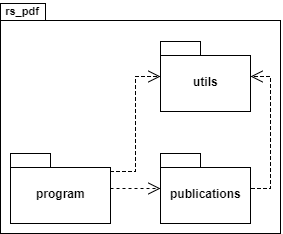
\includegraphics[scale=0.7]{figures/package.png}
\caption{Package diagram of RS\_PDF.}
\label{fig:package}
\end{figure}

In particular, the interaction with RS\_Server takes place within the package \textbf{program}. The server-side component itself can use the functionalities of RS\_PDF by executing it on the JVM, with a special set of command line options. Within this package, therefore, the parsing of the values received for each of these options and the management of the execution flow on the basis of these values take place.

The package \textbf{utils} has the task of providing useful tools to the remaining components of RS\_Rate. Inside it there are shared constants and methods that allow to access to the logging functionality. As it can be seen by looking at the diagram shown in Figure \ref{fig:package}, the other packages depend on it, in particular for some of the values of its constants.

The package \textbf{publications} contains the business logic to handle files encoded in PDF format that must be edited. Its classes follow the logic of the MVC pattern, although its exploiting is not bound by the used technology as in the case of an application developed with Rails. There is, therefore, a Controller which takes into account the execution parameters analyzed in the package \textbf{program} and updates the internal state of one or more instances of the Model which will be as many as the files encoded in PDF format that must be edited. This operation involves loading the input files and adding a link to RS\_Server on a new page, taking advantage of the functionalities of \emph{PDFBox}. As a last note, a View is not necessary because RS\_PDF simply saves the changes in a new PDF file and, then, ends its execution.

\subsection{Class Diagram}

Figure \ref{fig:classi-2} shows a diagram of the main classes of RS\_PDF which details the internal structure of the architectural elements outlined into the diagram shown in Figure \ref{fig:package}. The classes contained within the package \textbf{publications} are structured in a way which is similar to what Rails forces in RS\_Server and most of the processing carried out by RS\_Rate takes place within them. The Model contains the connections with PDFBox and its methods exploit these connections to actually edit files encoded in PDF format. 

A single exception to this structure is the use of the \emph{Parameters} class; in particular, it is only a \emph{data class}, i.e. a class whose sole purpose is to store data of various kinds. This instance, once created, is sent to the Model by the Controller through the interfaces of the Model itself. If it is necessary to send further data, the only thing to do consists in adding them to the data class, thus avoiding modifying the signatures of the methods of the Model. Regarding the contents of the \emph{program} and \emph{utils} packages, there is not much else to add with respect to what was said during the description of the diagram shown in figure \ref{fig:package}.

\begin{figure}[!tbp]
\centering
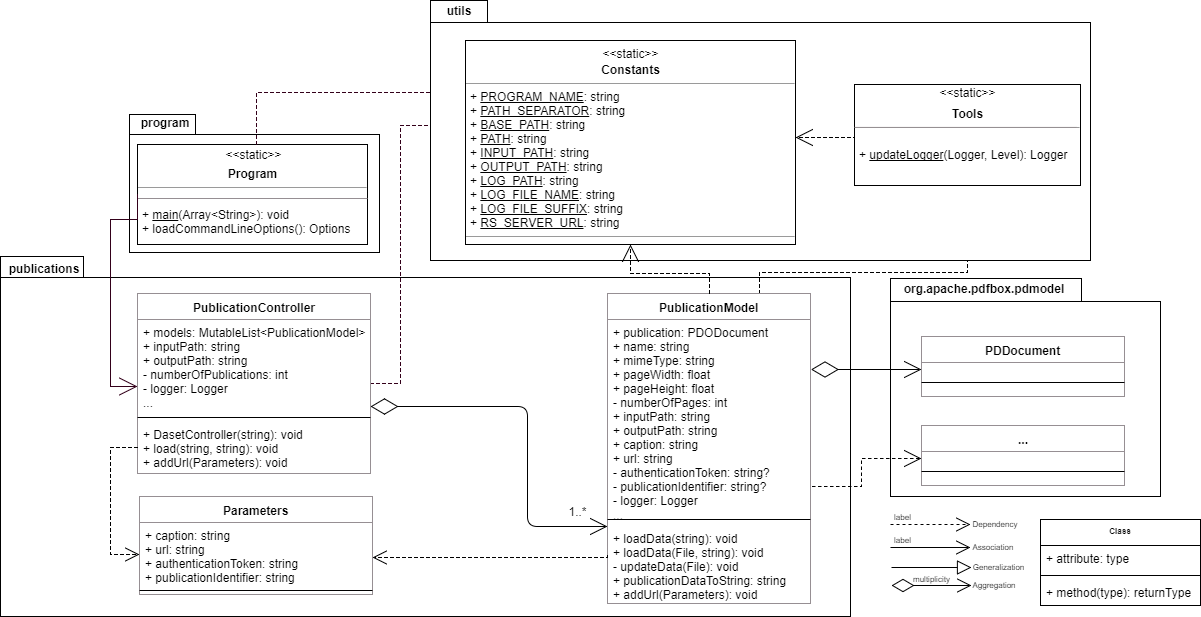
\includegraphics[scale=0.55, angle=90]{figures/classi-2.png}
\caption{Class diagram of RS\_PDF.}
\label{fig:classi-2}
\end{figure}

\subsection{Installation}

RS\_PDF comes bundled with RS\_Server, so when the latter is deployed there is no need to manually install the former. Nevertheless, it is possible to use it independently; it is sufficient to download the attached \verb|.jar| files from the release section of its repository\footnote{\url{https://github.com/Miccighel/Readersourcing-2.0-RS_PDF}} and place it somewhere on the filesystem.

\subsubsection{Requirements}

\begin{itemize}
\item JRE (Java Runtime Environment) $>=$ 1.8.0;
\end{itemize}

\subsubsection{Commmand Line Interface}

The behavior of RS\_PDF is configured during its startup phase by RS\_Server through a set of special command-line options. For this reason, it is useful to provide a list of all the options that can be used if it is necessary to use RS\_PDF in other contexts, modify its implementation or for any other reason. However, it is designed to work with a default configuration if no options are provided. This list of command line options in shown in Table \ref{tab:cli}. 
\begin{table}
\centering
\begin{threeparttable}
\begin{tabular}{p{1cm}p{2.4cm}p{3cm}p{3cm}p{1cm}p{1cm}}
\toprule
\textbf{Short}  &\textbf{Long} & \textbf{Description} & \textbf{Values} & \textbf{Req.} & \textbf{Deps.}  \\
\midrule
\verb|--pIn| & \verb|--pathIn | & Path on the filesystem from which to load the PDF files to be edited. It can be a file or a folder. & String representing a relative path. & No & \verb|--pOut| \\
\verb|--pOut| & \verb|--pathOut | & Path on the filesystem in which to save the edited PDF files. It must be a folder. & String representing a relative path. & No & \verb|--pIn| \\
\verb|--c| & \verb|--caption | & Caption of the link to add. & Any string. & Yes & No \\
\verb|--u| & \verb|--url | & Url to add. & A valid URL. & Yes & No \\
\verb|--a| &  \verb|--authToken| & Authentication token received from RS\_Server. & A valid authentication token received RS\_Server. & No & \verb|--pOut| \verb|--pIn| \verb|--pId|\\
\verb|--pId| &  \verb|--publicationId| & Identifier for a publication present on RS\_Server. & A valid publication identifier received from RS\_Server. & No & \verb|--pOut| \verb|--pIn| \verb|--a|\\
\bottomrule
\end{tabular}
\caption{Command line options of RS\_PDF.}
\label{tab:cli}
 \end{threeparttable}
\end{table}
To provide an execution example, let's assume a scenario in which there is the need of edit some files encoded in PDF format with the following prerequisites:
\begin{itemize}
\item there is a folder containing $n$ files to edit at path \verb|C:\data|;
\item the edited files must be saved inside a folder at path \verb|C:\out|;
\item the file in JAR format containing the library is called \verb|RS_PDF-v1.0-alpha.jar|;
\item the JAR file containing RS\_PDF is located inside the folder at path \verb|C:\lib|;
\item the authentication token received from RS\_Server is \\ \verb|eyJhbGciOiJIUzI1NiJ9....XpC9PMXOjtjRd4NBCtB1a4SfBEi6ndgqsE3k_cEI6Wo|;
\item the publication identifier received from RS\_Server is \verb|1|.
\end{itemize}
The execution of RS\_PDF is started with the following command:
\begin{lstlisting}
java -jar C:\lib\RS_PDF-v1.0-alpha.jar -pIn C:\data -pOut C:\out -a eyJhbGciOiJIUzI1NiJ9....XpC9PMXOjtjRd4NBCtB1a4SfBEi6ndgqsE3k_cEI6Wo -pId 1
\end{lstlisting}

\section{RS\_Rate}

\emph{RS\_Rate} is an extension for \emph{Google Chrome}\footnote{\url{https://www.google.com/chrome/}} and the client that readers actually use to rate publications; this means that every interaction with RS\_Server is carried out through this client. We intend to generalize RS\_Rate by providing an implementation for each of the major browsers (i.e., Firefox, Safari, \dots)

\subsection{Implementation and Technology}

RS\_Rate is an extension for Google Chrome; those extensions are developed using standard web technologies such as HTML, CSS and Javascript. Therefore, they are simple \lq\lq collections\rq\rq{} of files packaged in a CRX archive. This particular format is nothing more than a modified version of a ZIP archive with the addition of some special headers exploited by Google Chrome.

As for the Javascript component, RS\_Rate does not actually uses the \lq\lq pure\rq\rq{} language but instead uses jQuery, a library developed with the aim of simplifying the selection, manipulation, management of events and the animation of DOM elements in HTML pages, as well as implementing AJAX features. These AJAX features are widely used by RS\_Rate to improve the user experience during its use.

\subsection{Installation}

RS\_Rate is freely available on the main browsers webstores. To use it, simply take advantage of the following links and install the version for your favourite browser.
\begin{itemize}
\item \textbf{Google Chrome} version available at: \url{https://chrome.google.com/webstore/detail/readersourcing-20-rsrate/hlkdlngpijhdkbdlhmgeemffaoacjagg?hl=it};
\item \textbf{Firefox} version available at: \emph{currently disabled, will be available soon}.
\end{itemize}

\newpage

\printbibliography[heading=bibintoc]

\end{document}
